
\chapter{The objectives \& the data analysis process}

\section{Introduction}
The strategy is to cover data analysis applications over the three main goals. First, descriptive analytics aims to provide insight into what has happened. Second, predictive analytics helps to model and forecast what might happen. Thrird, prescriptive analytics seek to determine the best solution or outcome among various choices, given the known parameters.

Firstly, Pattern recognition applications that use machine learning algorithms to discover various patterns on operating pumping parameters using either supervised or unsupervised algorithms. Afterward, alarms and models are deployed that enables subject matter experts (SMEs) to unleash various behaviors downhole. Inferring real-time measurements using ground-truth values of previous sensors measurements or production tests lies also in this area of research. For instance, the technology of \ac{VFM} is considered one of the main applications in this area. 

The second strategy is predictive analytics. One of the main applications in this area is predictive maintenance. It mainly depends on detecting early signs in sensor measurements that exist by using machine learning and deep learning algorithms. 

Finally, Finally, dive into prescriptive analytics is introduced. It is referred to as the "final frontier of analytic capabilities". prescriptive analytics entails the application of mathematical and computational sciences and suggests decision options. For instance, predicting the optimum operating parameters (ie. pump frequency, injection rate..etc) in order to maximize the \ac{NPV}. Figure ~\ref{fig:Workflow} shows the whole data analytics startgies with their main objectives.  

\begin{figure}
    \centering
    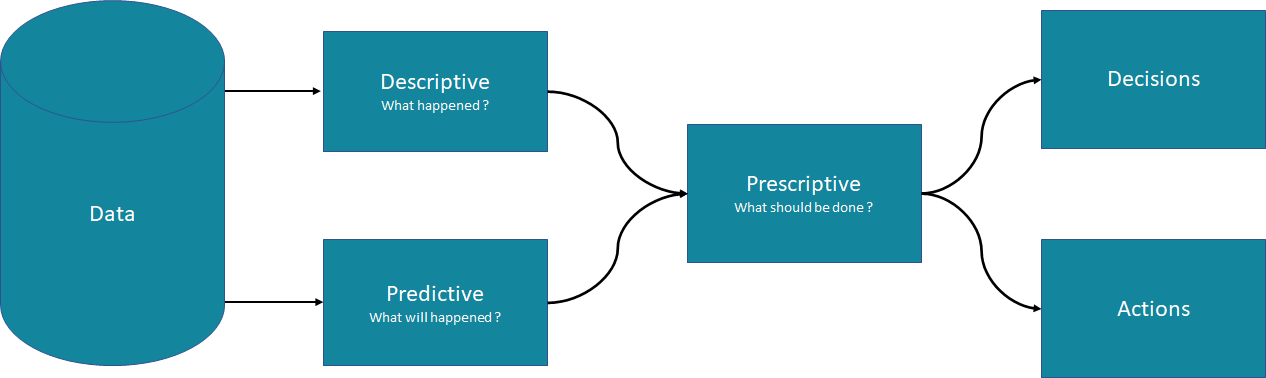
\includegraphics[keepaspectratio, width=\textwidth]{figures/workflow_design/workflowdesign.png}
    \caption{Workflow design}
    \label{fig:Workflow}
\end{figure}


\section{Objectives}

In the technological terms, this study aims to contribute to the area of data analytics in subsurface energy systems through the development of intelligent computing techniques. The developed applications targets the whole three stages of applications of data analytics. In other words, three different applications would be introduced. These applications are covering descriptive, predictive and prescriptive strategies. They are implemented using machine learning and deep learning algorithms on the oilfield data.

In the scientific terms, the main objective of this work is to develop three  models. First model should be able to predict oil production and water cut on wells that are deployed with electrical submersible pumps. It could be considered as an estimation of multiphase flow rates through wells. Second model would analyze the performance and unleash pattern between pre-event days (i.e. pre-workover days) and pump sensors measurements. The third model would be able to predict the optimum policy for injection rate in steam injection project.Table \ref{tab:workflowtable} presents a Summary of Projects and their relevant objective.

\begin{table}[]
    \centering
    \begin{tabular}{|p{3cm}|c|p{6cm}|}
        \hline
        Project & Area of Research & Objective \\ \hline
        Virtual flow meter for the \ac{ESP} & Descriptive modeling &  Real time inferring of oil rate and water cut of the \ac{ESP} wells using deployed pump sensors measurements \\     \hline
        Predictive maintenance of the \ac{ESP}  & Predictive modeling & Classify abnormal signals from 7 to 10 days before failure using rotated cloud of sensor data projected on principle axes  \\    \hline
        Steam injection rate optimization & Prescriptive modeling & Optimizing injection rate policy over time using actor critic reinforcement learning in order to maximizing the \ac{NPV}\\ \hline
    \end{tabular}
\caption{Summary of Projects and their relevant objective}
\label{tab:workflowtable}
\end{table}
   
\section{The data analysis process}
All of the aforementioned applications follow the process of data analysis applications. Basically all of them include understanding of the data then applying statistics to get insights for an engineering objective. Every study we would encounter is divided into four modules. Each module has a big impact on the overall performance of any problem. These four modules are:
•	Data gathering and exploratory data analysis
•	Feature extraction and transformation
•	Modeling 
•	Testing and Evaluation 

\subsection{Data gathering and exploratory data analysis}
Once the objective is established, A strategy is needed to be created for collecting and aggregating the appropriate data. This data might be quantitative (numeric) data, e.g. pump frequency for \ac{ESP}, stroke per minute for \ac{SRP}, or qualitative (descriptive) data, such as workover failure reason..etc In general, the training data set must include a number of cases from the aforementioned data. Each case contains values for a range of input and output variables.

Next step would be data cleaning. It is a crucial step because it enhance the quality data. Many tasks are included in data cleaning. Those are Removing major errors and duplicates, detecting outliers, and extracting irrelevant observations that have no bearing on the intended analysis. 

Likewise, It is important to carry out an exploratory data analysis. This helps identify initial trends and characteristics, and can even refine the hypothesis. It will give an idea of which inputs are likely to be influential. Exploratory data analysis helps to reveal hidden patterns, correlations, and anomalies using various tools such as visualizations (scatter and box plots, histograms, etc.), dimensionality reduction techniques and sometimes unsupervised algorithms for data grouping.

\subsection{Feature Extraction and transformation}
Feature extraction is one of the keys for a successful pattern recognition application. In definition, feature is a prominent part or characteristic of an object to distinguish itself. In machine learning application, the problem of large input data is encountered. The nature of input paramters could be in wave form or images presented as pixels. In such context, the input data can be transformed into a reduced set of features (also named a features vector). This process is called feature extraction. The selected features are expected to contain the relevant information from the input data. Hence, the desired task can be performed by using this reduced representation instead of the complete initial data.

In essence, feature extraction starts from an initial set of measured data. It builds derived values (features) intended to be informative and non-redundant. This facilitates the subsequent learning and generalization steps. 

\subsection{Modeling}
The type of data analysis is dependant upon the objective of the project. There are many techniques available. Univariate or bivariate analysis, time-series analysis, and regression analysis both linear and logistic could be considered as the fundamental studies for such modeling step. More important is how to apply them. This depends on the data itself and its complexity. Usually less to more complicated algorithms are applied in a sequence in order to unleash patterns inside the data. The inequality of explainability As described in DARPA’s research is that all AI techniques are not created equal in terms of their capacity for explainability. Complex algorithms requires recognition and careful consideration when using them for a particular use case. Figure \ref{fig:ml_explain} maps different types of AI systems according to their learning performance (i.e. accuracy) vs explainability. 

\begin{figure}
    \centering
    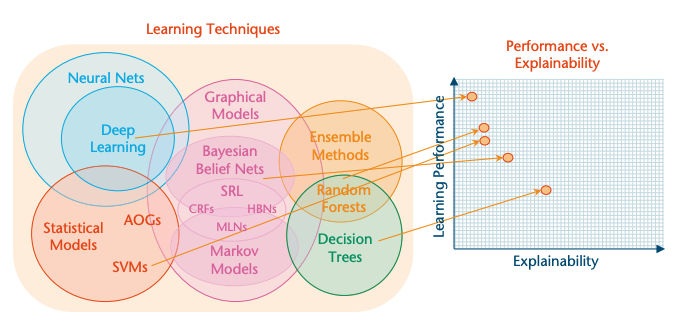
\includegraphics[keepaspectratio, width=\textwidth]{figures/workflow_design/perf_vs_expl.png}
    \caption{Algorithms inequality of explainability}
    \label{fig:ml_explain}
\end{figure}

Broadly speaking, all types of data analysis fit into one of the following three categories. When the data is prepared in desired format, Analytics would be performed which would give the insights for the relationship between sensor measurement, workover events and help in decision making. In these purposes, various algorithms could be used. These algorithms exhabit inverse relation between learning performance and explainability. Algorithms could range from Linear Regression, Clustering, Decision Tree techniques, support vector machines to come to a neural networks and deep neural learning.

\subsubsection{Descriptive analytics for Real time estimation and diagnostic modeling}
The objective of descriptive analysis here is to summarize the past row data to some models. These models are useful because they learn from past behaviors, and understand how they might influence future outcomes. The past row data refers to any point of time that an event has occurred, whether it is one minute ago, or one year ago. For instance, the sensor deployed data can be used to create model infer wells production. 

Diagnostic modeling focuses on understanding why something has happened. It is literally the diagnosis of a problem, just as the \ac{SME}s uses wells data to understand what happened downhole. For instance, it could help identifiying the condition of the sucker rod pump ug dynamomter cards.

\subsubsection{Predictive analytics for predictive maintenance}
Predictive analysis is used to identify future trends and forecasts accurately based on historical data. It has the ability to “predict” what might happen.
It has grown increasingly in recent years due to the evolution of machine learning and deep learning. It is of high importance to oil and gas industry because it helps in increasing production efficiencies through the proactive identification of failure events and the avoidance of deferment losses.

Predictive maintenance is a type of predictive anayltics that uses condition-monitoring sensor data to predict when equipment will fail. By predicting equipment failures, companies can schedule repairs during routine downtime. That enables them avoiding unplanned downtime and production loss. However, in many literature applications the term "predictive maintenance" is used interchangeably to refer to diagnostic modeling or operating data groupping.

Initiative, A key application in oil and geothermal energy systems would be developing an early failure Prediction model for artificial lift systems. In other words to be able to answer the question of when the well is going to fail?

\subsubsection{Prescriptive analytics for optimising manipulating parameters}
The Prescriptive analytics is a relatively new field. These analytics go beyond descriptive and predictive analytics by recommending one or more possible courses of action. It is used to “prescribe” a number of different possible actions and guide them towards an optimum  solution. It supports as advisory systems for the future. This is the final step in the analytics part of the process. It’s also the most complex. This is because it incorporates aspects of all the other analyses that have aforementioned.

Prescriptive analytics is a quite difference in application level. It use a combination of techniques and tools such as simulation studies, computational modelling procedures, and machine learning (ML).

A great example of prescriptive analytics is the algorithms that guide Google’s self-driving cars. Every second, these algorithms make countless decisions based on past and present data, ensuring a smooth, safe ride. Prescriptive analytics also helps in decision making for long term changes in manipulating paramters.

If it is implemented correctly, they could have a large impact on making decisions, and on the company’s bottom line. Technically, such analytics would contribute to the area of production optimization though making decsions on some maniulate parameters such as choke opening, pump frequency, injection rate and pump stroke per minute..etc.

In a nutshell, these analytics are all about providing advice. Prescriptive analytics attempts to quantify the effect of future decisions in order to advise on possible outcomes before the decisions are actually made. 

\subsection{Testing and Evaluation}
Model evaluation is very important in data science. It helps you to understand the performance of your model and makes it easy to present your model to other people. There are many different evaluation metrics out there but only some of them are suitable to be used for regression. This article will cover the different metrics for the regression model and the difference between them. Hopefully, after you read this post, you are clear on which metrics to apply to your future regression model.

Every time when I tell my friends: “Hey, I have built a machine learning model to predict XXX.” Their first reaction would be: “Cool, so what is the accuracy of your model prediction?” Well, unlike classification, accuracy in a regression model is slightly harder to illustrate. It is impossible for you to predict the exact value but rather how close your prediction is against the real value.

// regression modeling

Mean Absolute Error is the average of the difference between the Original Values and the Predicted Values. It gives us the measure of how far the predictions were from the actual output

Mean Squared Error(MSE) is quite similar to Mean Absolute Error, the only difference being that MSE takes the average of the square of the difference between the original values and the predicted values.

The cross plots of predicted versus actual data and calulating R square for this linear model
// classification modeling
The classification methods are evaluated and the best scenario of each algorithm has been chosen. Then, accuracy of each scenario is defined as the ratio of number of correctly classified reviews to the total number of reviews classified by the prediction model. Then, one of the two competitive algorithms was chosen for field applications validation. The results of the precision and recall measured for the proposed classification model is then discussed. This model evaluation is done for each rod pump conditions.

// unsupervised modeling (learning curve and ushape test)
The approach is to compute validation score of each cluster and then combine them in a weighted manner to arrive at the final score for the set of clusters. Let S be a set of clusters {C1 , C2 , C3 ,…………, Cn }, then validity of S will be computed as follows:

Cohesion for a cluster can be computed by summating the similarity between each pair of records contained in that cluster.

Separation between two clusters can be computed by summating the distance between each pair of records falling within the two clusters and both the records are from different clusters.

A set of clusters having high cohesion within the clusters and high separation between the clusters is considered to be good.

In practice, instead of dealing with two metrics, several measures are available which combine both of the above into a single measure. Few examples of such measures are:

Silhouette coefficient
Calisnki-Harabasz coefficient
Dunn index
Xie-Beni score
Hartigan index

Sofar in this blog series, we have looked at how to create automated playlists of songs by clustering a collection of tracks, based purely on their audio features. Previously, we worked on a toy example of 32 songs and showed how Hierarchical Agglomerative Clustering (HAC) can automatically create sub-groups of similar songs. We were able to verify the results of this clustering exercise through our existing knowledge of the songs (our algorithm confirmed that Motörhead and Black Sabbath are musically similar — go figure).

But what if we don’t have such prior knowledge of our data? What if the data isn’t even labelled (as is the case in many real-life clustering cases)? Even if it is, what if these labels are initially meaningless to us? There are plenty of artists that I’ve never even heard of, and if we’re trying to group thousands of tracks then it’s clearly impractical to manually verify every cluster. In these cases, we need some kind of mathematical measure for how ‘successful’ our clustering has been.

The Silhouette Score attempts to describe how similar a datapoint is to other datapoints in its cluster, relative to datapoints not in its cluster (this is aggregated over all datapoints to get the score for an overall clustering). In other words, it thinks about how ‘distinct’ the clusters are in space — indeed one could use any measure of ‘distance’ to calculate the score.

It is bounded between -1 and 1. Closer to -1 suggests incorrect clustering, while closer to +1 shows that each cluster is very dense.

// reinforcement learning modeling
Learning curve 
The learning curve is the plot of the magnitude or frequency of the conditioned response as a function of the number of reinforcements. Although conditioning has been studied for more

Challenge Due to both the mathematical sophistication and data-related concerns associated with statistical off-policy evaluation, other works choose to use more direct measures of policy performance. In this section, we consider a class of measures that we call the U-curve
method [Raghu et al., 2017, Prasad et al., 2017], which is based on the idea of associating
the difference between the clinician’s policy and the evaluation policy with some outcome,
such as mortality. If this association is positive, the reasoning goes, then it must mean that
when there is no difference—that is, when the clinician’s action agreed with the suggested
action—outcomes were the best.


\section{Summary}
Data Analytics is Storytelling, it tells you what is happening and what you should do to reach your objective.

we’ve covered the main steps of the data analytics process. These core steps can be amended, re-ordered and re-used as you deem fit, but they underpin every data analyst’s work:

Define the question—What business problem are you trying to solve? Frame it as a question to help you focus on finding a clear answer.
Collect data—Create a strategy for collecting data. Which data sources are most likely to help you solve your business problem?
Clean the data—Explore, scrub, tidy, de-dupe, and structure your data as needed. Do whatever you have to! But don’t rush…take your time!
Analyze the data—Carry out various analyses to obtain insights. Focus on the four types of data analysis: descriptive, diagnostic, predictive, and prescriptive.

Share your results—How best can you share your insights and recommendations? A combination of visualization tools and communication is key.
Embrace your mistakes—Mistakes happen. Learn from them. This is what transforms a good data analyst into a great one.

What next? From here, we strongly encourage you to explore the topic on your own. Get creative with the steps in the data analysis process, and see what tools you can find. As long as you stick to the core principles we’ve described, you can create a tailored technique that works for you.